\documentclass[english]{article}
\usepackage{graphicx}

\begin{document}



\title{Pascal to MIPs Compiler}
\author{Joseph Miller}
\maketitle


\section{Overview}

This program will be able to compile Pascal code into MIPs assembly code.  The compiler will be made divided into 5 major sections:

\begin{itemize}
\item
Scanner
\item
Parser
\item
Syntax Tree
\item
Semantic Analysis
\item
Code Generation
\end{itemize}


\par\addvspace{1cm}%
\section{Design}

\subsection{Scanner}

This program will be able to take in a file with Pascal code and output each token in the order that it was written. Each of the following keywords and symbols will be identified as tokens, as well as variable names (IDs).

enewcommand{\labelitemi}{$\textendash$}
\begin{itemize}
\item
\underline{Keywords:} and, array, begin, div, do, else, end, function, if, integer, mod, not, of, or, procedure, program, real, then, var, while
\item
\underline{Symbols:} ;, ,, ., :, [, ], (, ), +, -, =, \textless\textgreater, \textless, \textless=, \textgreater, \textgreater=, *, /, :=
\end{itemize}
This project is made of 3 Java/Class files:
\begin{itemize}

\item
\textbf{Scanner}: the DFA scanner made by JFlex to analyze the Paacal code and identify token types.
\item
\textbf{Token}: the token object creator, this file also takes in what kind of token it is and adds a more specific distinct type by using a look-up table (switch function / if-else function). Each Token object contains the lexeme and the type.
\item
\textbf{TokenType}: creates the specifications for a the TokenType attribute of the Token attribute
\end{itemize}
Illegal symbols and sequences not accepted by our simple pascal compiler will have the TokenType: ERROR. A visual of the tokens created can be seen in Figure ef{Output}, one of which produces an error.

\begin{figure}
\begin{center}
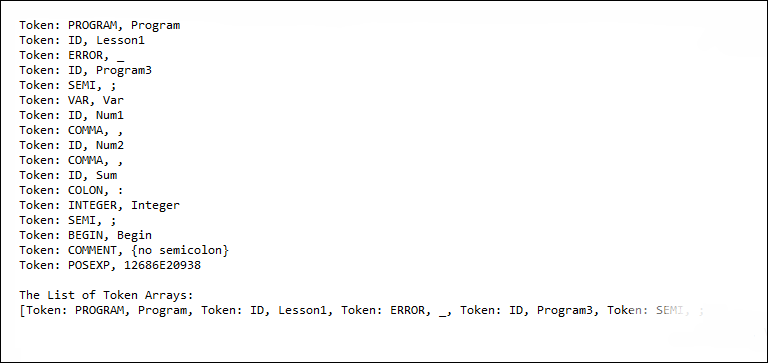
\includegraphics[width=1.1\textwidth]{output.PNG}
\end{center}
\caption{\label{Output}Token output to console}
\end{figure}


\subsection{Parser}

The parser takes the tokens from the scanner and verifies whether it is correctly formatted Pascal code. The parser also creates the syntax tree, a series of nodes that format the Pascal code for assembly code generation.

This project is made of 3 Java/Class files, only one of which (Parser) relates explicitly to the parser:

\begin{itemize}

\item
\textbf{Parser}: The parser class takes the series of tokens created by the scanner and uses functions for each production rule to either accept the Pascal code or reject it. If an error results it will also spot the location and reason for the error and end a message to the console informing the coder of the error. The parser adds identifiers to the symbol table with their proper type, and also uses the symbol table to resolves the ambiguity in the "Statement" production rule, where it calls either the "Procedure statement" or "Variable " production rule respectively. The parser also creates the syntax tree, using the classes in the syntax tree as nodes to construct a tree of the pascal code.

\item
\textbf{SymbolTable}: The symbol table is independent of the parser but is put in the parser package since the parser using it most and it’s not a large enough part of the compiler to be given its own package. The symbol table is used to take in all identifiers used in the code and associate them with the types of identifier (or symbol) they are. Other parts of the compilers will need to reference the symbol table.

\textbf{SymbolType}: This is an enum file for SymbolTable and has no relation to the parser itself. The five types of identifiers are: PROGRAMTYPE, VARIABLETYPE, FUNCTIONTYPE, PROCEDURETYPE, and ARRAYTYPE

\end{itemize}


\subsection{Syntax Tree}

The syntax tree package is a collection of classes that each represent a node in the syntax tree, and have methods and functions that connect to other nodes in the proper order. An example of some pascal code can be found in Figure ef{Tree Code} and the corresponding syntax tree code can be found in ef{Syntax Tree} These are the classes/nodes:

\begin{itemize}
\item
\underline{Nodes}: Assign, Assignment Statement, Compound Statement, Declarations, Expression, Function, If Statement, Operation, Procedure, Program, Read, Sign, Statement, Sub Program Declarations, Sub Program Head, Sub Program, Syntax Tree, Value, Variable, While Statement, Write
\end{itemize}



\begin{figure}
\begin{center}
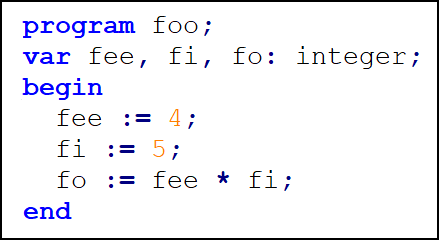
\includegraphics[width=.8\textwidth]{tree_code.PNG}
\end{center}
\caption{\label{Tree Code}Simple Pascal Code}
\end{figure}

\begin{figure}
\begin{center}
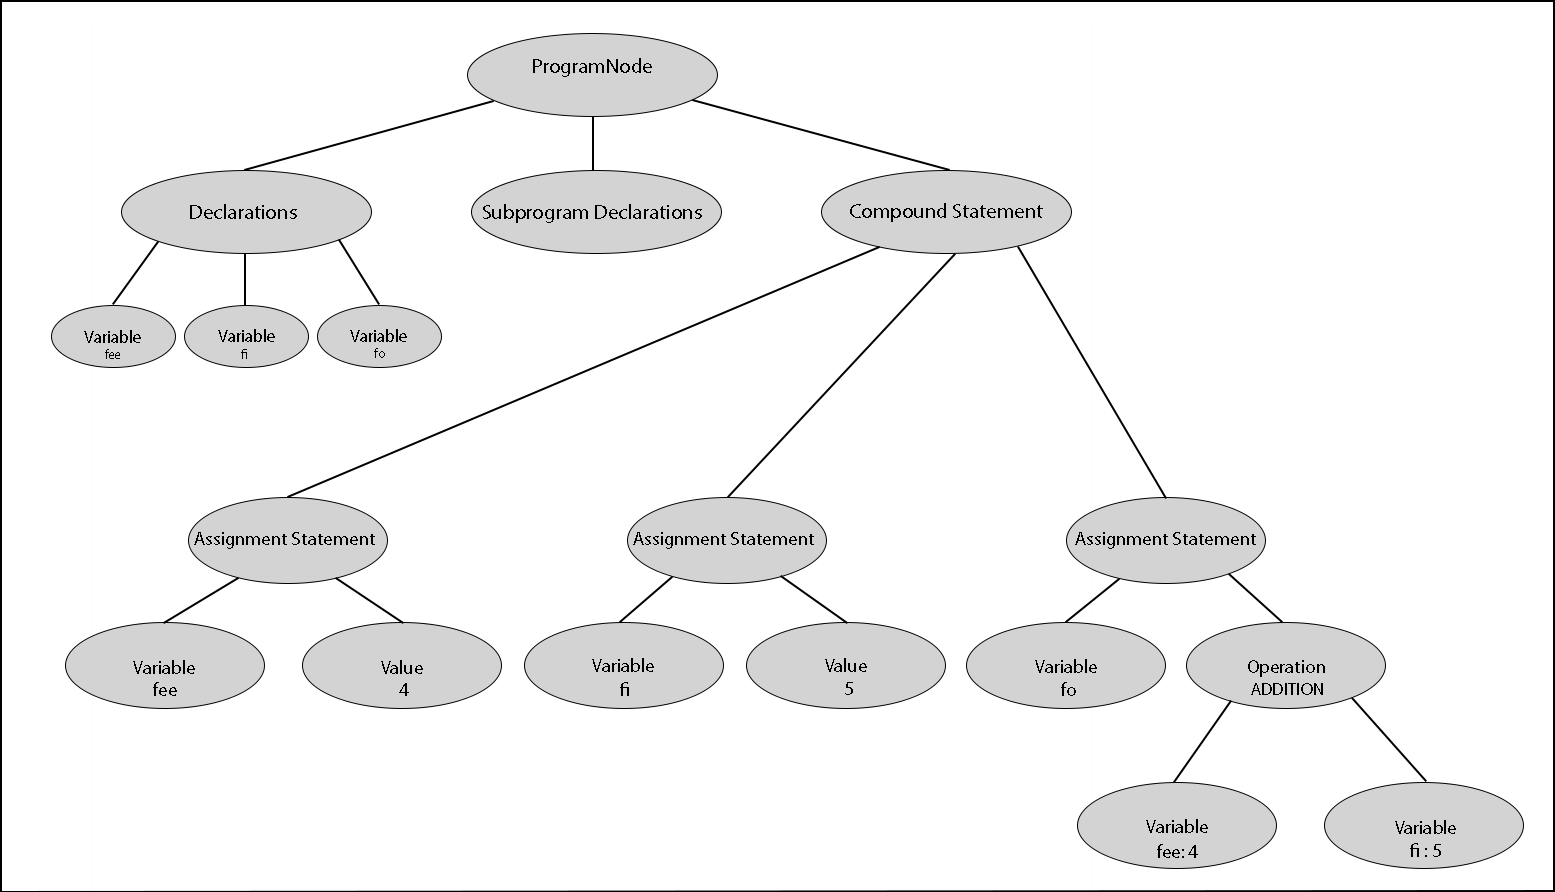
\includegraphics[width=1\textwidth]{syntax_tree.PNG}
\end{center}
\caption{\label{Syntax Tree}Syntax Tree Corresponding to Simple Pascal Code}
\end{figure}




\subsection{Semantic Analysis}

Not written

\subsection{Code Generation}

Not written



\par\addvspace{1cm}%
\section{Change Log}

\begin{itemize}
\item
18 January 2019 - Miller - Created
\item
3 Februrary 2018 - Miller - Added parser section and content
\item
11 February 2018 - Miller - Added symbol table info under parser section
\item
3 March 2018 - Miller - Added syntax tree section and content

\end{itemize}



\end{document}

